%%=================================================%%
%%						MAIN  
%%=================================================%%


\documentclass[a4paper]{report}

%====================== PACKAGES ======================
\usepackage{multirow}
\usepackage{bbold}
\usepackage{dsfont}
\usepackage[french]{babel}		% Pour avoir le document en français
\usepackage[utf8x]{inputenc}	% Encodage du document
\usepackage{float}				% Pour gérer les positionnement d'images
\usepackage{amsmath,,amssymb}
\usepackage{mathrsfs}			% Pour les lettres calligraphiques équation
\usepackage[colorinlistoftodos]{todonotes}
\usepackage{url}				% Pour faire des hyperliens vers le web
\usepackage{color}
% pour les informations sur un document compilé en PDF et les liens externes / internes
\usepackage{hyperref}			% Pour faire des hyperliens
\usepackage{array}				% Pour faire des tableaux
\usepackage{tabularx}
% pour utiliser 		% floatbarrier
%\usepackage{placeins}
%\usepackage{floatrow}

\usepackage{stmaryrd}
\usepackage{abstract}			% Modifier la mise en page de l'abstract
\usepackage[T1]{fontenc}		% Police et mise en page (marges) du document

\usepackage[top=2cm, bottom=2cm, left=2cm, right=2cm]{geometry}
\usepackage{pdfpages}			% pour inclures des pdf comme des images
\usepackage{subfig}				% Pour les galerie d'images
\usepackage{listings}			% pour inclure du code dans le doc
\usepackage{soul}				% Pour surligner
\usepackage{enumitem}
\sethlcolor{grisclair}
\definecolor{darkgreen}{RGB}{0,100,0}

\sethlcolor{grisclair}
\definecolor{darkgreen}{RGB}{0,100,0}
%% Titre import from last TP
\usepackage{titlesec, blindtext, color}	
\definecolor{gray75}{gray}{0.75}
\newcommand{\hsp}{\hspace{20pt}}
\titleformat{\chapter}[hang]{\Huge\bfseries}{\thechapter\hsp\textcolor{gray75}{|}\hsp}{0pt}{\Huge\bfseries}



%====================== INFORMATION ET REGLES ======================

%rajouter les numérotation pour les \paragraphe et \subparagraphe
\setcounter{secnumdepth}{4}
\setcounter{tocdepth}{4}

\hypersetup{							% Information sur le document
pdfauthor = {Johanne Bakalara, Lionel Merry, Alexandre , David Tocaven, Ibrahim Atto, Claire Paya, Lucien Rakotomalala},				% Auteurs
pdftitle = {Rapport Projet M2 ISTR },		% Titre du document
pdfsubject = {Analyse et commande robuste de procédés à événements discrets par des modèles non déterministes et des méthodes ensemblistes : application à la résolution de labyrinthes cartésiens variants, à dynamique ou mesure incertaine.},		% Sujet
pdfkeywords = {Automate, indéterministe,état discret, événement discret, SED, MEF, ambigus },				% Mots-clefs
pdfstartview={FitH}}					% ajuste la page à la largueur de l'écran
%pdfcreator = {MikTeX},% Logiciel qui a crée le document
%pdfproducer = {}} % Société avec produit le logiciel
 
\newcounter{cpt1}						% Compteur pour les n° de ligne dans les prog de l'annexe1
\newcommand\increm{\arabic{cpt1}\addtocounter{cpt1}{1}}
%======================== DEBUT DU DOCUMENT ========================

\begin{document}

%régler l'espacement entre les lignes
\newcommand{\HRule}{\rule{\linewidth}{0.5mm}}

%insertion image rapide
\newcommand{\image}[3]{\begin{center}
      \includegraphics[width = #1]{#2}
      \captionof{figure}{#3}
      \vspace{0.5cm}
\end{center}}

\newcommand{\imagegd}[6]{\begin{figure}[!ht]
\begin{minipage}{.48\textwidth}
\centering
\vfill%
\includegraphics[width = #1]{#2}
\caption{#3}\vfill%
\end{minipage}\hfill%
\begin{minipage}{.48\textwidth}
\centering
\vfill%
\includegraphics[width = #4]{#5}
\caption{#6}\vfill%
\end{minipage}
\end{figure}}

%page de garde
%%=================================================%%
%%						TITRE DU DOCUMENT (1 PAGE)
%							  Pas totalement fini
%%=================================================%%

\begin{titlepage}
\begin{center}

{\Huge\textbf{{\textsc{ State of art }}\\[.2cm]}}
\textit{\center{\Large  ``Analysis and robust control of discrete events process by non-deterministic model and set methods : application in Cartesian varying maze resolution,\break with uncertain dynamics or measures.''}\\[0.5cm]}
\end{center}
% Title :
%Analyse et commande robuste de procédés à événements discrets par des modèles non déterministes et des méthodes ensemblistes : application à la résolution de labyrinthes cartésiens variant, à dynamique ou mesure incertaine.



% Author and supervisor
\begin{minipage}[t]{0.4\textwidth}
\begin{flushleft} \large
\textbf{\large Authors :}\\%
\noindent\vspace{0mm}\\
\noindent\hspace{4mm}\begin{minipage}{.96\textwidth}
Johanne \textsc{Bakalara}\\
Claire \textsc{Paya}\\
Alexandre \textsc{Armengaud}\\
Lionel \textsc{Mery}\\
Lucien \textsc{Rakotomalala}\\
Ibrahim \textsc{Atto}\\
David \textsc{Tocaven}\\
\end{minipage}
\end{flushleft}
\end{minipage}\hfill%
\begin{minipage}[t]{0.38\textwidth}
\noindent\textbf{\large Supervisor :}\\
Yann \textsc{Labit}\\
Julien \textsc{Vanderstraeten}\\

 \vspace{1cm}
\textbf{\large Client :}\\
Sylvain \textsc{Durola}
\end{minipage}
\newline
\newline
\doublebox{
\begin{minipage}{.9\textwidth}
\vspace{1mm}
\underline{\textbf{\Large  Problematic}}\\
\label{chap:Intro}
\hspace{3mm}  \begin{minipage}{.96\textwidth}
\vspace{1mm}\hspace{2mm} The project focuses on the modeling and analysis with Discrete Events Systems (DES) of a system composed of a dynamic labyrinth and two objects moving inside the labyrinth.\\ This analysis will be used to identify properties to test this uncertain model.
We will contextualize our project with current knowledge in DES modeling.\\
First, we will redefine the definition of what we will call a "labyrinth" and then we will recall the formal definitions of DES \cite{controlOfDiscreteEvent_Ramadge} \cite{DiagnostabilityOfDES}.\\
In a second step, we will discuss more precisely the properties and products that we will use for the analysis and verification of our models. We will use the formal definitions explained in these books \cite{cassandras2009introduction} \cite{introductionAutomataTheoryLangageComputation_2007}. \\
The last part will remind us the scientific approach chosen and the types of verification and validation that will allow us to test our prototypes.
\end{minipage}

% Je dois contenir : 
% Problématiques (Comment peut on modéliser un labyrinthe ...

% Livre de départ : 
%%%%  Introduction to Discrete Event Systems :: Cassandras
% --> Infos utiles : 
% --> COmment l'a ton trouvé

%%%% An epistemic and dynamic approach to abductive reasoning: Abductive problem and abductive solution :: 

%%%% Stateless techniques for generating global and local test oracles for message-passing concurrent programs
\end{minipage}
}
% une éventuelle image
%\includegraphics[width=.6\textwidth]{./page_de_garde/BACDO_schema.pdf}~\\[1cm]

\vfill
\begin{figure}[hb]
\centering

\includegraphics[width=0.50\textwidth]{./page_de_garde/logo_ups.png}~\\[1cm]%
% Upper part of the page. The '~' is needed because only works if a paragraph has started.

\end{figure}
% Bottom of the page
\begin{center}
\large \today
\end{center}

%\end{center}
\end{titlepage}


%page blanche
\newpage
~
\tableofcontents
\thispagestyle{empty}
\setcounter{page}{0}
%ne pas numéroter le sommaire


%espacement entre les lignes d'un tableau
\renewcommand{\arraystretch}{1.5}

%====================== INCLUSION DES PARTIES ======================
%
%~
\thispagestyle{empty}
%recommencer la numérotation des pages à "1"
\setcounter{page}{0}

\doublebox{
\begin{minipage}{.9\textwidth}
\vspace{1mm}
\underline{\textbf{\Large  Problematic}}\\
\label{chap:Intro}
\hspace{3mm}  \begin{minipage}{.96\textwidth}
\vspace{1mm}\hspace{2mm} The project focuses on the modeling and analysis with Discrete Events Systems (DES) of a system composed of a dynamic labyrinth and two objects moving inside the labyrinth.\\ This analysis will be used to identify properties to test this uncertain model.
We will contextualize our project with current knowledge in DES modeling.\\
First, we will redefine the definition of what we will call a "labyrinth" and then we will recall the formal definitions of DES \cite{controlOfDiscreteEvent_Ramadge} \cite{DiagnostabilityOfDES}.\\
In a second step, we will discuss more precisely the properties and products that we will use for the analysis and verification of our models. We will use the formal definitions explained in these books \cite{cassandras2009introduction} \cite{introductionAutomataTheoryLangageComputation_2007}. \\
The last part will remind us the scientific approach chosen and the types of verification and validation that will allow us to test our prototypes.
\end{minipage}

% Je dois contenir : 
% Problématiques (Comment peut on modéliser un labyrinthe ...

% Livre de départ : 
%%%%  Introduction to Discrete Event Systems :: Cassandras
% --> Infos utiles : 
% --> COmment l'a ton trouvé

%%%% An epistemic and dynamic approach to abductive reasoning: Abductive problem and abductive solution :: 

%%%% Stateless techniques for generating global and local test oracles for message-passing concurrent programs
\end{minipage}
}	% 0.Introduction      

\chapter{Maze Definition} %this class ?
Our subject focuses on the modeling and analysis of a labyrinth, so we first presente a formal definition of a labyrinth throughout this state of art.\\ % Lucien ajout
We begin by using an existing definition: \textit{\textbf{"A maze is a grid-like two-dimensional area of any size, usually rectangular. A maze consists of cells. A cell is an elementary maze item, a formally bounded space, interpreted as a single site. The maze may contain different obstacles in any quantity."}} from \underline{Foundations of Learning Classifier Systems} by Larry BULL and T. KOVACS.
\\

In this definition, we can see the concept of dimension is important, it is introducing the notion of a cell. We chose to define a maze as a set of cells where the number of cells gives the dimension of a maze. This set of cell is confronting to all the obstacles that determines the possible and impossible paths. \\
In our study we are developing a maze with dynamics walls, an object trying to escape and a second one who is trying to find the first object. Each object choose a cell, he can go to the cell above, below, on the left or on the right depending on walls around him (they cannot cross the walls). So, a cell surrounded by four walls is not reachable and if an object is on, he is trapped. 

Now let us try to characterize our maze still based on paper from \underline{Anthony J. Bagnall and Zhanna V. Zatuchna } listed in the previous book.
%% ON NE PARLE PAS DU JEU PACMAN POUR NE PAS AVOIR PARLE DES CODES DEJA OPTIMISE POUR CE JEU, ON PARLE SIMPLEMENT D'OBJETS SE DEPLACANT DANS UN LABYRINTHE
\subparagraph{Size:}
2D rectangular with 25 cells (5x5)
\subparagraph{Distance from "Escape":} uncertain (short, medium, long)
\subparagraph{Obstacles:} moving walls, enemy (one object), edges of the maze
\subparagraph{Type of objects:} Object, Walls
\subparagraph{Maze Dynamics:} We have dynamics walls so our maze is called as \textit{dynamic maze}. A cell is reachable if there is no wall behind. If an object is on a cell, she is not reachable anymore by an other object.\\


% \textcolor{red}{on peut citer Dyna maze? elle à étudier les labyrinth dynamique c’est dans le livre  «Sutton R. S., Barto, A. G.: Reinforcement Learning: An Introduction. MIT (1998)» voila l’extrait «Dyna Maze. Consider the simple maze shown inset in Figure 9.5. In each of the 47 states there are four actions, up, down, right, and left, which take the agent deterministically to the corresponding neighboring states, except when movement is blocked by an obstacle or the edge of the maze, in which case the agent remains where it is. Reward is zero on all transitions, except those into the goal state, on which it is +1. After reaching the goal state (G), the agent returns to the start state (S) to begin a new episode. This is a discounted, episodic task with .» }

% %
% % 	ethimologie
% %	
% % 	De quel type ?
% A maze is a path or a collection of path typically from an start (entrance) point to a goal (escape).
% Generally, a maze can be defined in 7 classifications which are :
% \subparagraph{Dimension:}
% It's the dimension covered by our maze : we have a 2D Maze (5x5).
% \subparagraph{HyperDimension:} this class refers to the dimension of the moving object in the maze, we have two moving  small objects (Pacman and ghost), called a \textbf{non-hypermaze} case.
% \subparagraph{Topology:} this class describes the geometry of the space the maze exists in, we have a \textbf{Normal} standard maze in Euclidean space.
% \subparagraph{Tessellation:} this class refers to the geometry of the cells composing the maze : we have a regular rectangular grid where the objects can move, that type is called \textbf{Orthogonal}.
% \subparagraph{Routing} This class is By far, the most interissing in a maze because the main purpose of a maze is the routing, to find a successful way to the exit.
% For our system we have an object that can be in a dead end (four walls around it), it can also be in a loop or eaten by the second object: so it will be fair to say that we are in a \textbf{Partial Braid} maze case.
% A partial braid is a maze.
% \subparagraph{Texture} 
% % \textbf{symmetric:} A symmetric Maze has symmetric passages, e.g. rotationally symmetric about the middle, or reflected across the horizontal or vertical axis. A Maze may be partially or totally symmetric, and may repeat a pattern any number of times.\\
% % \textbf{elite:} The "elitism" factor of a Maze indicates the length of the solution with respect to the size of the Maze. An elitist Maze generally has a short direct solution, while a non-elitist Maze has the solution wander throughout a good portion of the Maze's area. A well designed elitist Maze can be much harder than a non-elitist one.\\
% % \textbf{bias:} A passage biased Maze is one with straightaways that tend to go in one direction more than the others. For example, a Maze with a high horizontal bias will have long left-right passages, and only short up-down passages connecting them. A Maze is usually more difficult to navigate "against the grain".\\
% % \textbf{run:} The "run" factor of a Maze is how long straightaways tend to go before forced turnings present themselves. A Maze with a low run won't have straight passages for more than three or four cells, and will look very random. A Maze with a high run will have long passages going across a good percentage of the Maze, and will look similar to a microchip.\\
% % \textbf{uniformity:} A uniform algorithm is one that generates all possible Mazes with equal probability. A Maze can be described as having a uniform texture if it looks like a typical Maze generated by a uniform algorithm. A non-uniform algorithm may still be able to potentially generate all possible Mazes within whatever space but not with equal probability, or it may take non-uniformity further in which there exists possible Mazes that the algorithm can never generate.\\
% % \textbf{river:} The "river" characteristic means that when creating the Maze, the algorithm will look for and clear out nearby cells (or walls) to the current one being created, i.e. it will flow (hence the term "river") into uncreated portions of the Maze like water. A perfect Maze with less "river" will tend to have many short dead ends, while a Maze with more river will have fewer but longer dead ends.} 
% We have a dynamic maze with mobile horizontal/vertical walls and a specific way of moving (walls->object1->object2) we can therefor say this is the texture of our maze.

% %%%%%%%%%%Je comprends pas !%%%%%%%%%%%%%%%
% \subparagraph{Focus:}
% This class shows that Maze creation can be divided into two general types: walls adders, and passage carvers.  The same Maze can be often generated in both ways.
% We  with the wall adders and added some vertical/horizontal matrices to define the states of our maze.\\
% \\
% Here's a little specifications on our maze environment

% \subparagraph{Specification}:\\
% 5x5 2D Maze (25 squares)\\
% Mobile Walls (dynamic)\\
% 1 exit
% \subparagraph{Object Specifications:}
% 2 object represented by a star that fit in the maze square, each object is in its own square anywhere on the maze at the initialization.
% Autonomous command or manual for both objects.

% \subparagraph{Rule}
% Pacman (object 1) who’s trying to escape and not get eaten\\
% Ghost (object2) who’s trying to eat Pacman\\
% One mouvement at a time and in a specific order (walls vertical or horizontal, Object1, Object 2)\\
% 2 object can’t be on the same square (position)
% Pacman has 2 lives (can be eat twice)\\
% Ghost can’t escape\\
% either one or both objects can be blocked


 % 1.Interface 2 joueurs

%\chapter{System}\label{System}

This part is an introduction to the concept of system in order to connect it to a labyrinth. We will find a complete definition obtained from scientist organizations and from our own meaning of system. 

\section{Definition}

The objective of this section is to give our definition of a system. The concept of system is explained with several primitives from multiple scientific and engineering organizations. We chose two of them :\begin{itemize}
\item "An aggregation or assemblage of things so combined by nature or man as to form an integral or complex whole" from \underline{Encyclopedia Americana
}.
\item  "A combination of components that act together to perform a function not possible with any of the individual parts" from  \underline{IEEE Standard Dictionary of Electrical and Electronic Terms}
\end{itemize} 

We chose to keep both definitions for two features : association of elements and the concept of function of a system. Therefore, for our next presentation, we will define a system as a collection of components which are interrelated in an organized way, and these associations work together for the accomplishment of some logical and purposeful ends. \label{definitionSystem}
%purposeful ?
% \section{Example and counter-example}  % Merci David .... -Lucien

\section{Modeling of System}\label{ModelingSystem}

Our initial approach for system modeling will be defined in this section. First, to enable analysis and command of our system, we have to respect the concept of input/output. In that way, it will be possible to describe mathematical behavior of our system by defining the outputs in function of input. To this end, we initiate a set of \emph{input variables} and \emph{output variables} \cite{cassandras2009introduction}, respectively $u(t)$ and $y(t)$, two vectors sizable $1\times p$ and $1\times m$:
\begin{align*}
&u(t) = \begin{pmatrix}
u_1(t)&...&u_p(t)
\end{pmatrix}^T \text{for }t \in [t_0, t_f]\\
&y(t) = \begin{pmatrix}
y_1(t)&...&y_p(t)
\end{pmatrix}^T \text{for }t \in [t_0, t_f]
\end{align*}

To enable a better representation of the system, we will add our modeling system the concept of state. This term consist in representing a set of variables named $x$, the present state of a system in $t\leq t_0$ and it will be used to calculate the set of outputs in $t$ and a next representation of this state, in $t + \tau$. This state vector is as defined below: 
\begin{align*}
&x(t) = \begin{pmatrix}
x_1(t)&...&x_n(t)
\end{pmatrix}^T \text{for }t \in [t_0, t_f]\\
\end{align*}

In addition, we would like to join the \emph{inputs}, \emph{outputs} and \emph{state variables} together that lead us to the concept of \emph{state space} (sections 1.2.6 of \cite{cassandras2009introduction}). Here are relationships between $u$, $y$ and $t$ if the vector of \emph{state variables} is correctly chosen. It refers to the \emph{dynamics} of the system and it can take a few possible representations, but we chose to present you this one, it seems to us to be the most complete one:
\begin{eqnarray} \label{equationSystem_1}
\left\lbrace
\begin{aligned}
&\dot{x}(t)= f(x(t), \delta, u(t), t)\\ %Mega boulette de ma part, sorry...
&y(t) = h(x(t), \delta, u(t), t) 
\end{aligned} 
\right.
\end{eqnarray}

 %vérifier le sens  // C'est mieux ? -Lucien 
The first function $f$ represents the system dynamics using a differential equation of the system state variable. The second function $g$ models the output exigences. We have modeled various parameters thanks to this equation. Here is the list : \begin{itemize}
\item $\delta \in \Delta$ incertitude of the system, we chose not to forget the potentially unknown and instable parameters of the system.
\item $t \in \mathbb{R}^{+}$ evolution of time of some parameters.
\end{itemize} 

These types of system modeling are called nonlinear, variant and non deterministic system with continuous time. They are not suitable for mathematical analysis (although possible) or control. Assumptions are then imposed to remove non-linearity, variability and non-determinism through computational steps so as not to stray too far from the complex model.

Many methods exists to simplify this complex model; they will not be detailed here, we will see later that the theoretical assumptions on the models will enough. We just have to remember that each hypothesis added on the complex model yields: \begin{itemize}
\item \underline{Linearization} gives a model defined by:
\begin{eqnarray} \label{equationSystem_Linear}
\left\lbrace
\begin{aligned}
&\dot{x}(t)= A(t, \delta)x(t) + B(\delta, t)u(t)\\ %Mega boulette de ma part, sorry...
&y(t) = C(t, \delta)x(t) + D(\delta, t)u(t) 
\end{aligned} 
\right.
\end{eqnarray} with the linearization of $f$ and $g$ on two linear composition $A$ and $B$ for $f$ and $C$ and $D$ for $g$.
\item \underline{Invariant} prevents the model from being time-dependent:
\begin{eqnarray} \label{equationSystem_Invariant}
\left\lbrace
\begin{aligned}
&\dot{x}(t)= f(x(t), \delta, u(t))\\ %Mega boulette de ma part, sorry...
&y(t) = g(x(t), \delta, u(t)) 
\end{aligned} 
\right.
\end{eqnarray} Here we simplify the elements that were based on time, i.e. it could change instantly. This hypothesis means the following model is invariant.
\item \underline{Deterministic} We associate the uncertainties within the system with some elements of the system:
\begin{eqnarray} \label{equationSystem_Invariant}
\left\lbrace
\begin{aligned}
&\dot{x}(t)= f(x(t), u(t), t)\\ %Mega boulette de ma part, sorry...
&y(t) = g(x(t), u(t), t) 
\end{aligned} 
\right.
\end{eqnarray} Uncertain parameters are now associated with reliable parameters, we have an approximation of our model: it is named deterministic.
\end{itemize}

Now we propose this assumption, let's look at the shape of the state space model. This one is described below, and called \emph{Deterministic Continuous Time Invariant Linear System}: 
\begin{eqnarray} \label{equationSystem_DCTIL}
\left\lbrace
\begin{aligned}
&\dot{x}(t)= Ax(t) + Bu(t)\\ %Mega boulette de ma part, sorry...
&y(t) = Cx(t) + Du(t)
\end{aligned} 
\right.
\end{eqnarray}

In the next step, we will see a subclass of this type of systems, where continuous time is not an evolutionary variable anymore. System-class called Discrete Time System exists. The evolution is based on a sample sequence $kTe$ with $k\in \mathbb{N}$ the sample number and $Te \in \mathbb{R}$ a sample frequency and another sub-class, the Discrete Event System, where the sampling frequencies only dependent upon events which are now presented. % 2.Interface 1 joueur

\chapter{Commandes} \label{sec:commandes}

Dans un premier temps nous avons créé des commandes intuitives que nous avons implémentées dans les classes dédiées ($ModelPacman$, $ModelGhost$ et $ModelWalls$). Les commandes intuitives sont détaillées ci-après. Dans la suite du projet nous en avons créé de nouvelles plus performantes, qui remplaceront celles-ci.

\section{Commandes de pacman} \label{sec:commandePacman}
%Intuitives: 
\subsection{Avec priorité}
Cette commande vérifie si elle peut aller à droite (pas de mur) sinon en bas, sinon à gauche, sinon en haut :\\
\image{7cm}{3_Commandes/commande_pacman_simple}{Commande simple de Pacman}
\subsection{Avec mémoire}
Cette commande garde en mémoire un vecteur à 4 entrées. L'entrée 1 passe à 1 si on a fait droite, l'entrée 2 à 1 si on a fait bas, l'entrée 3 à 1 si on a fait gauche, l'entrée 4 à 1 si on a fait haut. Une fois qu'on a testé les quatre possibilités, le vecteur est remis à 0.\\
Sa représentation complète sous forme automate est très conséquente (environ 120 états), vous la trouverez dans le code dans le dossier $laby\_1\_player\_automaton$, en voici une partie pour donner une idée :
\image{11cm}{3_Commandes/commande_pacman_memory}{Commande Memory de Pacman}

\section{Commandes de ghost}\label{sec:commandeGhost}
\subsection{Ghost voit Pacman}
Avec cette commande si ghost voit pacman dans son couloir (aucune séparation par des murs) il va dans sa direction. S'il ne le voit pas il fonctionne avec une priorité (haut, bas, gauche, droite).
\subsection{Ghost ne reste pas bloqué}
Cette commande respecte les mêmes conditions que précédemment mais prend aussi en compte qu'il ne peut pas aller sur une case dans laquelle il pourra se retrouver bloqué au prochain tour. S'il ne voit pas ghost ou que si là ou il le voit il peut se retrouver bloqué, il suit la même règle de priorité que précédemment, toujours en évitant la case bloquante.\\
\\
Ces commandes n'ont pas été modélisées, car il faut les adapter au procédé complet avec deux objets.

\section{Commandes des murs}\label{sec:commandeMurs}
Les murs verticaux peuvent seulement se déplacer vers le bas et les murs horizontaux vers la droite.
\subsection{Alternée}
Les murs horizontaux se déplacent à leur tour, puis les murs verticaux au tour d'après. Ils alternent donc à chaque tour de jeu.
\image{5cm}{3_Commandes/commande_murs.png}{Commande des murs alternée}
\subsection{Une fois sur deux}
Les murs ne se déplacent qu'une fois sur deux et de façon alterné comme précédemment. Attention cette commande n'est pas compatible avec la commande de "ghost ne reste pas bloqué". En effet, ghost n'a pas accès aux informations du labyrinthe, il connait juste la situation initiale et leur commande, il calcule donc la prochaine position des murs (il ne la lit pas!). Cette commande de ghost a été conçue pour fonctionner avec la première commande de mur.

\image{5cm}{3_Commandes/commande_murs.png}{Commande des murs une fois sur deux}

 % 3.Commandes

\chapter{Automaton}

%%%%%%%%%%%%%%%%%%%%%%%%%%%%%%%%%%%%%%%%%%%%%%%%%%%%%%%%%%%%%%%%%%%%%%%%%%%%%
\section{Definition and Representation of an Automaton}
A finite automaton is a Finite State System composed of discrete inputs and outputs. It is a mathematical model of system composed of a finite number of states. Each state summarize informations and the configuration of these states determine the behavior of the system. We could for example model a human brain with a finite state system considering that each neuron contains informations which can be described by a small number of bits. Furthermore the number of neurons is limited to $2^{35}$ at most.\\
We consider an automaton as a set of states and transitions from state to state that occur on input symbols. We can model the system as a graph, called a \textit{transition diagram} which is associated with a finite automaton. The verticals of the graph correspond to the states of the finite automaton. Each state is modeled by an unique circle labeled and transitions are modeled by an arrow from one state to another one that is also labeled. An event can occur many times but a state is unique.\\
This definition is inspired by the book \textit{introduction Automata Theory Langage and Computation} written by John E Hopcroft, R.Motwani and Jeffrey D.Ullman. \cite{introductionAutomataTheoryLangageComputation_2007}\\

\subsubsection*{For example : A light}
We model a light that starts and switch on off if one press the button :
\begin{center}
      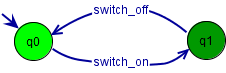
\includegraphics[width = 5cm]{./IV/ex1.png}
      \captionof{figure}{\label{automate}Example 1 - finite automaton}
      \vspace{0.5cm}
\end{center}

This automaton is composed of :
\begin{itemize}
\item two states : {q0,q1}
\item an initial state : {q0}
\item two transitions : {switch\_off, switch\_on}
\end{itemize}

In a maze context, objects and the dynamics walls have a behavior we can model with automaton. The object moves can have as possible transitions $up$, $down$, $left$, $right$, the walls can also have moves, $up$, $down$, $left$, $right$. Each cell of our maze is a state where few events can occur. For example, each possible event that can happen on every cell - if we don't know the position of the object - is described by the next automaton \ref{maze} :

\begin{figure}[H]
\begin{minipage}{0.5 \textwidth}	
      \begin{center}
      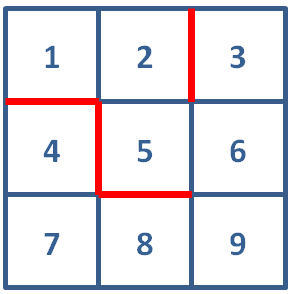
\includegraphics[width = 3cm]{./IV/3x3lab.png}
      \caption{Example - Maze}
      \end{center}
\end{minipage}
\begin{minipage}{0.5 \textwidth}
\begin{center}
      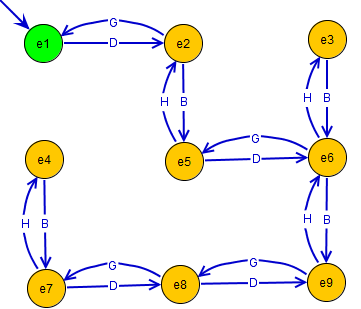
\includegraphics[width = 4cm]{./IV/3x3autom.png}
      \captionof{figure}{\label{maze} Example - Automaton }
      \end{center}
\end{minipage}
\end{figure}


\section{Formal representation of an deterministic automaton}
We formally denote a finite automaton by the next 5-tuple :
\begin{equation}
\mathcal{A} = ( Q, \Sigma,\delta,q_0,F )
\end{equation}

With :

\begin{tabular}{lll}
$Q$ & : & finite set of states.\\
$\Sigma$ & :& finite input alphabet.\\
$q_0$ & :& $q_0 \in Q$ the initial state.\\
$F$ & :& $F \subset Q$ the set of final states\\
$\delta$ & :& the transition function mapping $Q$ x $\Sigma$ to $Q$
\end{tabular}\\
\begin{description}
\item [Alphabet :] set of all events known by the automaton
\item [String :] one sequence of transitions
\item [The transition function :] a string x is accepted by the automaton $\mathcal{A}$  if $\delta(q_0,x)=p$
\end{description}


%%%%%%%%%%%%%%%%%%%%%%%%%%%%%%%%%%%%%%%%%%%%%%%%%%
%Rajouter ref vers la bliblio
\section{Formal representation of a nondeterministic automaton}
As explained by Hopcroft, Motwani and Ullman \cite{introductionAutomataTheoryLangageComputation_2007}, \textit{"a nondeterministic automaton has the power to be in several states at once"}. In the formalization we supposed that a same input can arrive to several states. The definition of an automaton remains mainly the same.
\begin{equation}
\mathcal{A} = ( Q, \Sigma,\delta,q_0,F )
\end{equation}

With :

\begin{tabular}{lll}
$Q$ & : & finite set of states.\\
$\Sigma$ & :& finite set of input alphabet.\\
$q_0$ & :& $q_0 \in Q$ the initial state.\\
$F$ & :& $F \subset Q$ the set of final states\\
$\delta$ & :& the transition function mapping $Q$ x $\Sigma$ to $\mathcal{P}(Q)$
\end{tabular}\\

The difference between a nondeterministic and a deterministic automaton is the type of value that $\delta$ returns. Thus, the transition function is extended : \\
\begin{equation*}
w=xa
\end{equation*} where $a$ is the final letter of $w$ and $x$ is the rest of $w$
\begin{equation*}
\widehat{\delta}(q,x)=\{p_1,p_2,...,p_k\}
\end{equation*}
\begin{equation*}
\bigcup_{k}^{i=1}\delta(p_i,a) = \{r_1,r_2,...,r_m\}
\end{equation*}
Then \begin{equation*}
\widehat{\delta}(q,w) = \{r_1,r_2,...,r_m\}
\end{equation*}

Cassandras define nondeterministic finite automata as \cite{cassandras2009introduction}:
\begin{equation*}
\widehat{\delta} : Q × \Sigma \rightarrow 2^X
\end{equation*}
\begin{equation*}
\widehat{\delta}(x, s) \subseteq Q
\end{equation*}
with
\begin{equation*}
q_0 \subseteq Q.
\end{equation*}

\subsection{Language Notation and Definitions}
Definition (Language and notation, \cite{cassandras2009introduction})  : A language defined over an event set $L$ is a set of finite-lenght strings formed from events in E.\\
As an example, let $\Sigma=\{a, b, g\}$ be the set of events. We define a language :
$L=\{\epsilon, a, abb\}$.\\
The definition of the language for an automaton is really useful to analyze it. Language is a mathematical tool used to do operations, in order to extract many properties for automata. We recall how to express the language of an automaton then the operations below.

%%%%%%%%%%%%%%%%%%%%%%%%%%%%%%%%%%%%%%%%%%%%%%%%%%%%%%
\subsection{Languages Represented by Automata}
Definition by Cassandras\cite{cassandras2009introduction} :\\
The language generated by $ A = ( Q, \Sigma,\delta,q_0,F )$ is :
\begin{equation*}
\mathcal{L}(A) := \{ s \in \Sigma^* \delta(q_0,s) \text[is \hspace{0.1cm} defined] \}
\end{equation*}


The language marked by $A$ is :
\begin{equation}
\mathcal{L}_m(A) := \{ s \in \mathcal{L}(A) : \delta(q_0, s) \in F\}
\end{equation}
with the extended transition function : $\delta : Q$ × $\Sigma ^{∗} \rightarrow F $ with $\epsilon \in \mathcal{L}(A)$\\

%Lien entre language et automates
The language generated by $A$ represents all strings existing in the automaton starting at the initial state. The string is the concatenation of the event labels of the transitions for a path in an automaton. It is also called a sequence.\\
The marked language represents all strings ending at a marked state. We also said that the language is \textit{recognized} by the automaton.

\textbf{\underline{For instance :}} \\
      \begin{center}
      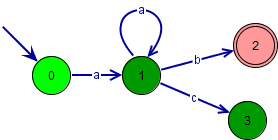
\includegraphics[width = 5cm]{./IV/ex2.png}
      \captionof{figure}{Automaton example}
      \end{center}
      
This finite state automaton is $\mathcal{A} = (Q, \Sigma,\delta,q_0,F )$  with :
\begin{itemize}
\item $Q=\{0,1\}$
\item $\sigma = \{a,b,c\}$
\item $q_0 = {0} $
\item $F=\{2\}$
\item $\delta(0,a)=1$, $\delta(1,a)=1$, $\delta(1,b)=2$, $\delta(1,c)=3$
\end{itemize}

We can see from the figure and the definitions that :
\begin{itemize}
\item $\mathcal{L}_m (A)=aa*b$
\item $\mathcal{L}_g (A)=aa*(b+c)$
\end{itemize}


% \begin{equation*}
% \mathcal{L}(G) = \{s \in E^* : (\exists q \in q_0) [\delta(q, s) \text[is\hspace{0.1cm}defined] ]\}
% \end{equation*}
% \begin{equation*}
% \mathcal{L}(G) = \{s \in \mathcal{L}(G) : (\exists q \in q_0)[\delta(q, s) \cap F = \emptyset]\}
% \end{equation*}

We formally define the language for a deterministic automaton as :\\
\begin{equation*}
L(\mathcal{A}) = \{x|\delta(q_0,x) \cap F\}
\end{equation*}

if a state is accepted by the one finite automaton, it is a \textit{regular set} \\
\\
The language accepted by the nondeterministic finite automaton is defined by : 
\begin{equation*}
L(\mathcal{A}) = \{w|\widehat{\delta}(q_0,x)\} \cap F \neq \emptyset
\end{equation*}
If a main sequence of choices from a start state to any accepting state if possible, it accepts a string $w$ .

%%%%%%%%%%%%%%%%%%%%%%%%%%%%%%%%%%%%%%%%%%%%%%%%%%%%%%%%%%%%%%%%%%%%
\subsection{Operations} 

Let's consider two languages $L$ and $M$ and an alphabet $E$.\\
\begin{description}
\item [Union] : $L \cup M$ set of strings which are in the languages $L$ or $M$.
\item [Concatenation] : the concatenation of L and M is detoned by a "dot" or nothing as $L.M$ or $LM$. $LM$ contains each string in $L$ concatenated with each string in $M$. Each string must only appear once. The empty string $\epsilon$ is the identity element : $u \epsilon = \epsilon u = u$
\end{description}
\begin{equation*}
L,M \subseteq E^*
\end{equation*}
\begin{equation*}
LM := \{s \in E^*: (s = s_Ls_M) and (s_L ∈ La) and (s_M \in L_M)\}
\end{equation*}

\begin{description}
\item [Kleene-closure/ Kleene star] : it is denoted $L^*$, any number of possible strings  with repetitions, concatenating all, including the empty string $\epsilon$.
\end{description}
\begin{equation*}
L \subseteq E^*
\end{equation*}
\begin{equation*}
L^∗ := {\in} \cup L \cup LL \cup LLL \cup ...
\end{equation*}

\begin{description}
\item [Projection] : 
\end{description}

\begin{equation*}
L \subseteq E_l^*
\end{equation*}
\begin{equation*}
P(L) :=\{ t \in E_s^* : (\exists \in L) [P(s)=t] \}
\end{equation*}

\begin{equation*}
L \subseteq E_s^*
\end{equation*}
\begin{equation*}
P^{-1}(L_s) := \{ s \in E_l^* : (\exists t \in L_s) [P(s)=t] \}
\end{equation*}

\begin{description}
\item [Example of operations for Languages] : $E=\{a,b\}$ and $L =\{c, acb, abc, cacacb, aacbcab\}$
\item\hspace{6.6cm} Consider the projection : $ P: E_l^* \rightarrow E^*$\\
\end{description}

\begin{center}
$P(L) = \{ \epsilon, ab, aab, aabab\}$ \\
$P^{-1}(\{\epsilon\}) = \{c\}^*$\\
$P^{-1}(\{b\}) = \{c\}^*{b}{c}*$
\end{center}



%%%%%%%%%%%%%%%%%%%%%%%%%%%%%%%%%%%%%%%%%%%%%%%%%%%%%%%%%%%%%%%%%%%%%%%%%
\subsection{Properties}
The properties below were extracted by the operations.
\begin{description}
\item [Language-equivalent automata \cite{cassandras2009introduction} ] : Automata $G_1$ and $G_2$ are said to be language-equivalent if
$\mathcal{L}(G_1) = \mathcal{L}(G_2)$ and $\mathcal{L}_m(G_1) = \mathcal{L}_m(G_2)$ \\

\item [Blocking] : Automaton $G$ is said to be blocking if $ \mathcal{L}_m(G_1) \subset\mathcal{L}(G) $
and nonblocking when $ \mathcal{L}_m(G_1) \subset \mathcal{L}(G) $

\item [Accessibility] : A state is said $accessible$ a sequence/word exists from the initial state to this state. With the definition $\mathcal{L}(G)$ and $\mathcal{L}_m(G)$ explained above, we can apply them to find all existing words from the initial state to all reachable states :
\end{description}


\begin{equation*}
A_{ac} = \{q \in Q | (\exists s \in \Sigma^∗) [\delta(q_0, s) = q]\}
\end{equation*}

\vspace{0.5cm}

An automaton is defined as \emph{accessible} if all its states are accessible : $Ac(A)=Q$.\\
Despite as it is explained in \cite{cassandras2009introduction} by \textit{Cassandras and Lafortune}, we will consider that an accessible state  is not necessarily marked by $\mathcal{A}$.

\begin{description}
\newpage
\item [Coaccessibility] : A state is named $coaccessible$ a sequence/word it exists from this state to a marked state. With the definition $\mathcal{L}(G)$ and $\mathcal{L}_m(G)$ explained above we can apply them in order to find all existing words from all states to one of the marked states :
\end{description}

\begin{equation*}
C_o(A) = \{q_j \in Q| \exists s \in \Sigma^* \text[avec] \delta(q_j, s) \in F\}
\end{equation*}
 \vspace{0.5cm}
 
An automaton is defined as $coaccessible$ if all its states are coaccessible : $C_o(A)=Q$. Thus, $\mathcal{L}(G) = \overline{\mathcal{L}_m(G)}$\\
Coaccessibility is closed to the concept of blocking : an automaton is $blocked$ if $\mathcal{L}(G) \neq \overline{\mathcal{L}_m(G)}$. It means, states do exist that are accessible but not coaccessible.

\subsection{Composition Operations}
Two types of operations for deterministic automata exist : product and parallel composition. They can be directly be applied in classical methods on the graph but it comes from the language operations.\\ 
Product composition between two automata lets show the synchronization on a common event. An event can occur if it is in both Automata but it also contains the independent event of each automaton. We formally defined the product of $G_1$ and $G_2$ as the automaton : 
\begin{equation*}
G_1 \times G_2 := A_c (Q_1 \times Q_2, \Sigma_1 \cap \Sigma_2, \delta, Q_{m1} \times Q_{m2})
\end{equation*}
\begin{equation*}
\mathcal{L}(G_1 \times G_2) = \mathcal{L}(G_1) \cup \mathcal{L}(G_2)
\end{equation*}
\begin{equation*}
\mathcal{L}_m(G_1 \times G_2) = \mathcal{L}_m(G_1) \cup \mathcal{L}_m(G_2)
\end{equation*}
 In a \textit{parallel composition} an event can only  occur if both automata execute it simultaneously : they are synchronized.
 The parallel composition of $G_1$ and $G_2$ is the automaton :
 \begin{equation*}
 G_1 \parallel G_2 := Ac ( Q_1 \times Q_2,\Sigma_1 \cup \Sigma_2, \delta, F_1\times F_2)
 \end{equation*}
 \begin{equation*}
 \mathcal{L}(G1\parallel G2) = P_1^{-1}  [\mathcal{L}(G1)] \cap P_2^{-1}  [\mathcal{L}(G2)]
 \end{equation*}
 \begin{equation*}
 \mathcal{L}_m(G1\parallel G2) = P_1^{-1}[{L}_m(G1)] \cap [P_2^{-1}{L}_m(G2)]
 \end{equation*}
 
 %%%%%%%%%Faire un exemple%%%%%%%%%%%%%%%%%%%%%%%
 
 \subsection{Modeling a system with Automata - Inspired by the Supervisory Command}
 %Citation
The model that describes all existing situations of a system and its behavior (events, inputs, outputs, states) is called \textit{The process model}. If we want to choose a specific behavior of this system, we have to create a a model that describes these objectives. If we need to reach these objectives (for instance : "arrive in a marked state "), we must to create a model that describes these objectives. It is usually called \textit{the objectives command}.\\
The \textit{Composition Operation} of both models describes the appropriate behavior because it only contains the common events from both models. This new model is called the \textit{Command model}.\\
In our context, all events are observable and controllable, so Cassandras explains the usefulness for using the parallel composition or the product :\\
\textit{The choice of product or parallel composition to compose [the specification model] called $H_{spec}$ with [the process Model called] $G$ is based on the events that appear in the transition diagram of $H_{spec}$ and on how we wish to define the event set of $H_{spec}$} :
\begin{itemize}
\item \textit{ If the events that can be executed in G but do not appear in the transition diagram of $H_{spec}$ are irrelevant to the specification that $H_{spec}$ implements, then we use parallel composition and define the event set of $H_{spec}$ to be those events that appear in its transition diagram.}
\item \textit{ On the other hand, if the events that can be executed in G but do not appear in the transition diagram of $H_{spec}$ are absent from $H_{spec}$ because they should not happen in the admissible behavior $L_a$, then product is the right composition operation.}
\end{itemize}
\textit{ Equivalently, parallel composition can still be used provided the event set of $H_{spec}$ is defined carefully and includes the events that should be permanently disabled.\\
 In most cases, all the states of $H_{spec}$ will be marked so that marking in [the result of the operation] $H_a$ the will be solely determined by G.}
 
 %%%%%%%%%%%%%%%%%%%%%%%%%%%%%%%%%%%%%%%%%%%%%%%%%%%%%%%%%%
 \section{Implementation by sequential system blocks}
 The automota can be implemented by a sequential system because the evolution of the system depends on the present state, the next state but also of inputs and outputs of the system. The implementation based on a Moore Machine is a formal way to implement automota. 
 %include MOOR MACHINE
 \begin{figure}[!ht]
       \begin{center}
      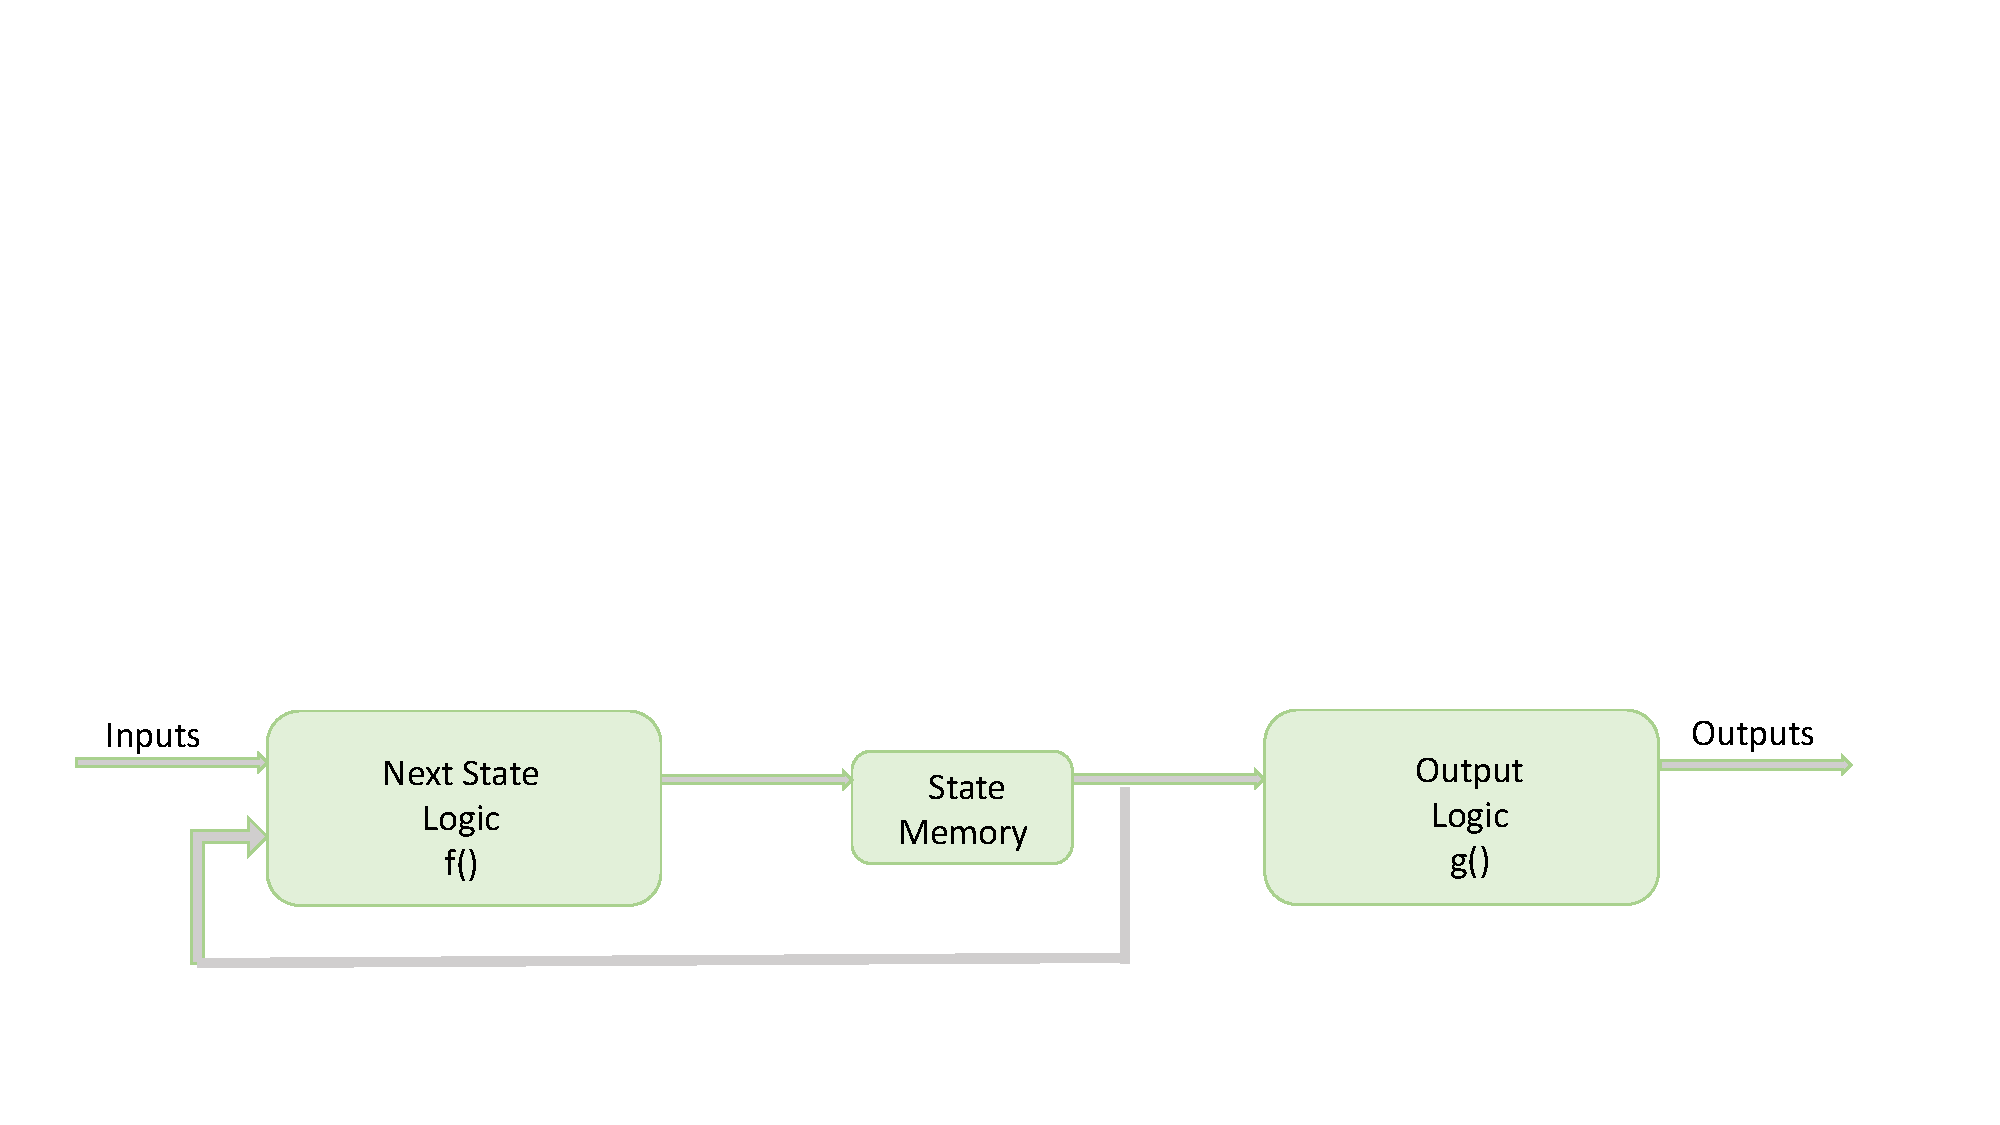
\includegraphics[width = 18cm]{./IV/schema_FMG.pdf}
      \end{center}
  \end{figure}
  
 We define the next state with our transition function, we memorize the present state and generate the outputs and then we define the new next state with the present state and the new inputs.\\
 It's adapted to be implemented in different languages. Our project uses the language object Matlab implementation, where each class has a present State containing his intern situation and his own evolution functions $f()$, $m()$ and $g()$ that read the inputs, calculate outputs and the next State.






 % 4.Vérifications

\chapter{Verification and validation}

\section{Approach methods}

%A comprendre
%We chose to study three principal types of approaches. They are adapted according to the research carried out (fundamental or applied). This part consists of presenting these types of reasoning.
We chose to study three types of approaches. There are adapted for researches and development fundamental or applied. During our project we shall use the next three approaches by using theoretical proofs or validation tests. This part consists of introducing these different types of reasoning.
% Nous avons choisi d'étudier trois types principaux d'approches. Ils sont adaptés en fonction des recherches effectuées (fondamentales ou appliquées).Durant notre projet, nous aurons l'occasion de les utiliser en trouvant des preuves théoriques ou en réalisant des test de validation. Cette partie consiste à présenter ces types de raisonnement.

\subsection{Inductive Approach}
%An inductive approach begins with observation and then generalizes to broader theories \cite{o2004essential}.
%This reasoning is divided in four steps, it is necessary to begin with the observations for then analyze these observations. For finally generalize in the form of hypotheses and verify them.
An inductive approach begins by observing of our system used to generalize our theories.[Wilson, J. (2010) “Essentials of Business Research: A Guide to Doing Your Research Project” SAGE Publications, p7] \cite{buisnessREsearchWilson}\\
This reasoning is composed of four steps :
\begin{itemize}
\item Observing
\item Analyzing the observations
\item Generalizing thanks to hypothesis
\item Verifying hypothesis
\end{itemize}
% Une approche inductive commence par l’observation pour ensuite généraliser sur des théories plus large [Wilson, J. (2010) “Essentials of Business Research: A Guide to Doing Your Research Project” SAGE Publications, p7]. 
% Ce raisonnement est divisé en quatre étapes, il est faut commencer par des observations pour ensuite analyser ces observations. Pour enfin généraliser sous la forme d'hypothèses et de les vérifier.

\subsection{Deductive Approach}
%Deductive reasoning involves testing a theory and seeking confirmation through observations\cite{o2004essential}. We can thus prove and explain implicit relationships of cause and effect.
%The deductive approach generally takes place in four stages, at first it must deduce hypotheses from the theory, for then test these hypotheses and analyze the results. Depending on these results, the theory can be modified.
The deductive reasoning consists in testing a theory then confirming if throw the analysis of the observations  [Wilson, J. (2010) “Essentials of Business Research: A Guide to Doing Your Research Project” SAGE Publications, p5] \cite{buisnessREsearchWilson}\\
We can prove and explain implied a cause to effect relationships.
This reasoning is composed of four steps :
\begin{itemize}
\item Deducing hypothesis from theory
\item Testing hypothesis
\item Analyzing results %sous forme d'hypothèse
\item Modifying theory if necessary
\end{itemize}
% Le raisonnement déductif consiste à tester une théorie et à rechercher une confirmation par des observations  [Wilson, J. (2010) “Essentials of Business Research: A Guide to Doing Your Research Project” SAGE Publications, p5]. On peut ainsi prouver et expliquer des relations implicite de cause à effet. 
% L'approche déductive se déroule généralement en quatre étapes, pour commencer, il faut déduire des hypothèses de la théorie, puis tester ces hypothèses et analyser les résultats. En fonction de ces résultats, la théorie peut être modifiée.

\subsection{Abductive Approach}
%The abductive reasoning is to give explanations to an experiment and to obtain a hypothesis. This reasoning is often used in the areas of scientific discovery, legal reasoning and diagnosis because it is said to be conducive to innovation. Overall, abductive reasoning can be viewed as a process of four phases:
%First, we must recognize the existence of an abductive problem. Secondly, candidate solutions must be identified. Third, choose the most plausible solutions. Fourth, assimilate the solutions chosen \cite{VELAZQUEZQUESADA2013505}.
The abductiv reasoning consists in finding explanations of an experiment and hypothesis. It is used for scientific discoveries because it is more convenient to innovative approaches. As explained by Wilson, the abductiv approach contains four steps :
\begin{itemize}
\item Recognizing the existence of an abductiv problem
\item Identifying solutions
\item Finding possible solutions
\item Explaining solutions and implementing them to solve the problem %eexpliquer ces solutions et savoir les mettre en œuvre pour résoudre le problème rencontré
\end{itemize}

% Le raisonnement abductif consiste à donner des explications à une expérimentation et à obtenir une hypothèse. Ce raisonnement est souvent utilisé dans le domaine de la découverte scientifique car il est particulièrement adapté à des approches  innovantes. En référence à l’article cité, le raisonnement abductif peut être perçu comme un processus contenant quatre phases :
% Premièrement, il faut reconnaitre l’existence d’un problème abductif. Deuxièmement, il faut identifier les solutions candidates. Troisièmement choisir les solutions les plus plausibles. Quatrièmement, assimiler les solutions retenues.

\section{Test method}
% Afin de valider le code, la mise en place d'une méthode de vérification et de validation du code est nécessaire, il est notamment possible d'utiliser des oracles . Ces oracles permettent de verifier la réussite ou l'echec d'un test. C’est à dire de déterminer si le résultat obtenu à l'issu du test correspond bien au resultat attendu \cite{CARVER2018237}.\\
% Plusieurs cas de test doivent être abordés, en fonction des scénarios désirés. Ces cas de test correspondent à des données de test à mettre en place en entrée de l'oracle. En sortie de ce dernier, le resultat confirmera la validitée ou non du code testé. Ces cas de tests peuvent avoir une approche soit inductive en réalisant une multitude de tests soit abductive en réalisant des test précis et ciblés pour chaque cas critique.

%%%% DeepL and Johanne translation ;) %%%%%%%%%%%%%%%%%%%%%%%
%verifier comment on traduit validation et abductif
In order to validate the code, it is necessary to set up a method of verification and validation of the code, it is notably possible to use \textit{oracles}. An oracle is a small code that runs along the code. It is used to verify the success or failure of a test. It means, we should determine if the result obtained at the end of the test corresponds to the expected one \cite{CARVER2018237}.
Several types of tests are needed, it depends on an expected scenarios. These types of tests correspond to data tests that must be sent at the oracle input. At the output of the oracle, the result will confirm the validity or invalidity of the tested code. These test cases can either have an inductive approach by performing a multiply tests or an abductive approach by performing precise and targeted tests for each critical case.





 % 5.Analyse

\chapter{Le petite guide d'utilisation}

\section{Organisation du code}
A l'ouverture du dossier principal on trouve quatre sous dossiers :

\begin{itemize}
\item Doc : contenant la documentation rattachée au projet (rapport, état de l'art et la doc générale )
\item Src : contenant le code
\item UML : contenant l'UML du code (voir le READ ME)
\end{itemize}
\image{15cm}{6_Code/GUIDE}{Arborescence du dépôt}

\section{Comment lancer l'interface ?}
Il y a deux interfaces : celle à 1 objet et celle à 2 objets.\\
Pour lancer celle à 2 objets, on ouvre le dossier \emph{Laby2players} et on lance le fichier \emph{main}. Pour tout ce qui se rapporte à son utilisation, se référer au chapitre 1 - Interface \ref{chap1}\\
Pour lancer l'interface à 1 joueur, on ouvre le dossier \emph{laby1player} et on lance le fichier \emph{main}. Pour tout ce qui se rapporte à son utilisation, se référer au chapitre 1 - Interface \ref{chap1}.

\subsection{Comment changer la figure ?}
La figure est modifiable avec \emph{figure\_laby.fig} mais implique beaucoup de changements au niveau de \emph{figureLaby;m}, du \emph{Wrapper} et du code en règle général. Se référer au chapitre 1 \ref{chap1} pour le fonctionnement global du code.

\subsection{Comment changer l'ordonnancement ?}
Il est possible de changer l'ordonnancement depuis le \emph{Wrapper} (valable pour les deux interfaces). Comme précédemment, se référer au chapitre 1 \ref{chap1}

\subsection{Comment changer la commande des objets ?}
Il est possible d'implémenter ses propres commandes pour pacman, ghost ou les murs dans leur fonction respective : ModelPacman, ModelGhost, ModelWalls qu'on trouve dans les deux dossiers \emph{Laby1player} et \emph{Laby2players}. Se référer au chapitre 2 sur les commandes pour l'explication de l'implémentation \ref{commandes}.

\section{Comment lancer les validations logicielles ?}
Les validations ont été faites pour l'interface à 2 joueurs. On ouvre le dossier  \emph{Laby2players}, puis le dossier de validation. Chaque dossier de validation contient l'oracle à faire tourner sur la première version du code.\\
Le code affiche en ligne de commande s'il y a un problème ou non. Pour cette partie une seconde interface a été créée, une vidéo de tous les coups ou des 100 premiers coups est générée automatiquement dans le but de pouvoir observer visuellement certains cas particuliers. Cette vidéo est enregistrée dans le dossier \emph{data}. La fonction vidéo existe également pour la version à 1 objet. Dans les deux cas on lance le fichier \emph{simulation}. Se référer au chapitre 3 - Vérification et Validation pour plus de détails \ref{verif}.

%ajouter quelle version

\section{Comment lancer la validation formelle ?}
La validation formelle a été réalisée pour un joueur. On va donc dans le dossier \emph{Laby1player} puis on ouvre le dossier \emph{automaton} duquel on lance le \emph{main}. De là un menu s'affiche dans lequel on choisit la commande à valider.\\
Le code renvoie s'il existe des séquences et si oui lesquelles pour atteindre l'état marqué. La saisie du labyrinthe étudié se fait dans le dossier \emph{modelGenerator}, dans le fichier \emph{modelGenerator.m}. Attention la position initiale est toujours fixée à la case 1. Se référer au chapitre 3 pour plus de détails \ref{verif}.

\subsection{Comment générer le procédé indépendamment ?}
Le modèle de procédé est calculé directement en fonction du labyrinthe donné dans le dossier \emph{modelGenerator} dans le fichier \emph{modelGenerator.m}. Si vous souhaitez le générer indépendamment, il faut aller dans le dossier \emph{modelGenerator} et lancer le fichier \emph{modelGenerator.m} puis le raffiner avec la fonction \emph{rafineAutomaton.m}. Se référer au chapitre 3 pour plus de détails \ref{verif}.

\subsection{Comment valider ma propre commande ?}
Si vous créez votre propre commande, il faut la créer sous Desuma et l'enregistrer sous le format \emph{.fsm} et l'enregistrer dans le dossier \emph{automaton}. Attention le langage doit être en accord avec le langage connu du procédé et lors de la saisie sous Desuma les états doivent être nommés avec des numéros (par exemple : 1 et non e1 ou état1). Pour plus de détails se référer au chapitre2 - Les commandes \ref{commandes}.\\
Une fois la commande enregistrée lancer le \emph{main} normalement et suivez les indications du menu.
\image{15cm}{6_Code/automaton}{Exécution du produit parallèle pour la vérification et le scénario 1}


\section{Comment lancer le scénario 1 ?}
Le scénario 1 est prévu pour 1 objet, on se place dans le dossier \emph{laby1player} puis on ouvre le dossier \emph{automaton} duquel on lance le fichier \emph{main}. C'est le même code que précédemment sauf qu'on utilise le produit parallèle pour trouver une commande pour un objectif et non pour valider une commande. Du menu qui s'affiche on choisit l'objectif à atteindre.\\
Le code renvoie s'il existe une séquence et si oui, la plus optimale pour atteindre l'objectif.

\subsection{Comment tester mon propre objectif ?}
Même démarche que pour \textit{Comment valider ma propre commande ?}.

\section{Comment lancer le scénario 2 ?}
Le scénario 2 est prévu pour 1 objet, on se place dans le dossier \emph{laby1player} puis on ouvre le dossier \emph{automaton\_nd} duquel on lance le fichier \emph{main}. Un menu s'affiche pour choisir l'ensemble d'états initiaux et l'état marqué.\\
Le code renvoie la séquence pour atteindre l'état marqué. Voir le chapitre 4 - Les scénarios pour plus de détails \ref{sce}.

\section{Comment lancer le scénario 3 ?}
Il ne fonctionne pas encore mais la génération automatique de modèle a commencé à être codé dans le sous dossier \emph{ModelGenerator} de \emph{Laby2players}. % 6.Code

\chapter{Conclusions}








%Ne pas numéroter cette partie
\part*{Annexes}
%Rajouter la ligne "Annexes" dans le sommaire
\addcontentsline{toc}{part}{Annexes}

%\chapter*{Annexe 1 - TITRE}
\addcontentsline{toc}{chapter}{TITRE}
%\setcounter{section}{0}
% **********************************
\addcontentsline{toc}{section}{TITRE}
\label{Annex:NOM_FICHIER}
\lstset{
  language=Matlab,                	  % choose the language of the code
  basicstyle=\ttfamily,
  numbers=left,                   % where to put the line-numbers
  stepnumber=1,                   % the step between two line-numbers.
  numbersep=5pt,                  % how far the line-numbers are from the code
  backgroundcolor=\color{white},  % choose the background color. You must add \usepackage{color}
  commentstyle = \color{darkgreen},
  showspaces=false,               % show spaces adding particular underscores
  showstringspaces=false,         % underline spaces within strings
  showtabs=false,                 % show tabs within strings adding particular underscores
  tabsize=2,                      % sets default tabsize to 2 spaces
  captionpos=b,                   % sets the caption-position to bottom
  breaklines=true,                % sets automatic line breaking
  breakatwhitespace=true,         % sets if automatic breaks should only happen at whitespace
  %caption=exo1.m,                 % show the filename of files included with \lstinputlisting;
  literate={á}{{\'a}}1 {è}{{\`e}}1 {é}{{\'e}}1,
}
%\lstinputlisting{./annexes/annexe1/NOMFICHIER.m} %{language = MAtlab}	




\end{document}